\documentclass{article}
\usepackage[a4paper, portrait, margin=1.1811in]{geometry}
\usepackage[english]{babel}
\usepackage[utf8]{inputenc}
\usepackage[T1]{fontenc}
\usepackage{helvet}
\usepackage{etoolbox}
\usepackage{graphicx}
\usepackage{titlesec}
\usepackage{caption}
\usepackage{booktabs}
\usepackage{xcolor} 
\usepackage[colorlinks, citecolor=cyan]{hyperref}
\usepackage{caption}
\captionsetup[figure]{name=Figure}
\graphicspath{ {./images/} }
\usepackage{scrextend}
\usepackage{fancyhdr}
\usepackage{graphicx}
\newcounter{lemma}
\newtheorem{lemma}{Lemma}
\newcounter{theorem}
\newtheorem{theorem}{Theorem}

\fancypagestyle{plain}{
	\fancyhf{}
	\renewcommand{\headrulewidth}{0pt}
	\renewcommand{\familydefault}{\sfdefault}
	%\rhead{p-ISSN: 693-7554 \\ e-ISSN:2654-3990}
	%\rfoot{\thepage} --> Show the page number
	
}

%\pagestyle{plain}
\makeatletter
\patchcmd{\@maketitle}{\LARGE \@title}{\fontsize{16}{19.2}\selectfont\@title}{}{}
\makeatother

\usepackage{authblk}
\renewcommand\Authfont{\fontsize{10}{10.8}\selectfont}
\renewcommand*{\Authsep}{, }
\renewcommand*{\Authand}{, }
\renewcommand*{\Authands}{, }
\setlength{\affilsep}{2em}  
\newsavebox\affbox

\author{Proud Jiao}
\author{Xiaocong Xuan}
\author{Yijie Lu}
\author{Xiaoyan Wei}
\author{Lukas Lam}
\author{Felix Zhou}

\affil[]{ Statistics Department, UCLA
}


\titlespacing\section{0pt}{12pt plus 4pt minus 2pt}{0pt plus 2pt minus 2pt}
\titlespacing\subsection{12pt}{12pt plus 4pt minus 2pt}{0pt plus 2pt minus 2pt}
\titlespacing\subsubsection{12pt}{12pt plus 4pt minus 2pt}{0pt plus 2pt minus 2pt}


\titleformat{\section}{\normalfont\fontsize{10}{15}\bfseries}{\thesection.}{1em}{}
\titleformat{\subsection}{\normalfont\fontsize{10}{15}\bfseries}{\thesubsection.}{1em}{}
\titleformat{\subsubsection}{\normalfont\fontsize{10}{15}\bfseries}{\thesubsubsection.}{1em}{}

\titleformat{\author}{\normalfont\fontsize{10}{15}\bfseries}{\thesection}{1em}{}

\title{\textbf{\huge Indications of Heart Failure}\\
 }
\date{}    

\begin{document}

\pagestyle{headings}	
\newpage
\setcounter{page}{1}
\renewcommand{\thepage}{\arabic{page}}


	
\captionsetup[figure]{labelfont={bf},labelformat={default},labelsep=period,name={Figure }}	\captionsetup[table]{labelfont={bf},labelformat={default},labelsep=period,name={Table }}
\setlength{\parskip}{0.5em}
	
\maketitle 
	
\noindent\rule{15cm}{0.5pt}
	\begin{abstract}
	The main question we wanted to answer is what are significant indicators that could predict heart failures. The methods we used include Exploratory Data Analysis (EDA) to find patterns and especially correlations between predictors and heart failure and ANOVA to determine statistical evidence for correlation. The results indicate that common indicators such as Age, Sex, Resting Blood Pressure, Fasting Blood Sugar Level, and Max Heart Rate, all have significant correlations with heart disease. 
	\end{abstract}
 
\noindent\rule{15cm}{0.4pt}

\section{Introduction}

Heart Disease is the leading cause of death within the US, with one person dying every 34 seconds due to a heart related issue. Up to 90\% of these deaths are preventable, but a mere 8\% of Americans recognize this (CDC).
We wanted to take the initiative and find out the leading symptoms that indicate heart disease.

Our research question is, for Heart Failure, what factors increase the chances of being diagnosed for heart failure? We will take a look at various predictors, within the Heart Disease data set, and closely examine the correlation between predictors and whether heart failure is present. Additionally, we validate our statistical findings with credible medical sources, such as Mayo Clinic and Center for Disease Control (CDC). 



\section{Background}

We preformed our statistical analysis on the Heart Disease data set, which includes 368 different observations and 60 different predictors. However, we narrowed our predictors to more common indicators such as, Age, Sex, Resting Blood Pressure, Fasting Blood Sugar Level, and Max Heart Rate. 

In our statistical analysis, we encoded those that are positive for heart disease as 1, or commonly displayed as a blue color, and 0 for those that are negative for heart disease, or commonly displayed as a red color. 
Following the encoding for positive or negative for heart disease, we also encoded a Fasting Blood Sugar Level < 120 mg/dl as red, and a Fasting Blood Sugar Level > 120 mg/dl as blue.


\section{Methods | Exploratory Data Analysis}
\subsection{Correlation Matrix}
We first investigated the general trend of correlation between predictors using the correlation matrix\ref{fig1}. The last column in this graph specifically shows correlations between heart failures and other predictors. For example, MaxHR has a negative correlation with heart failure, and fasting blood sugar level has a positive correlation with heart failure, etc.

\begin{figure}[h]
	\centering
	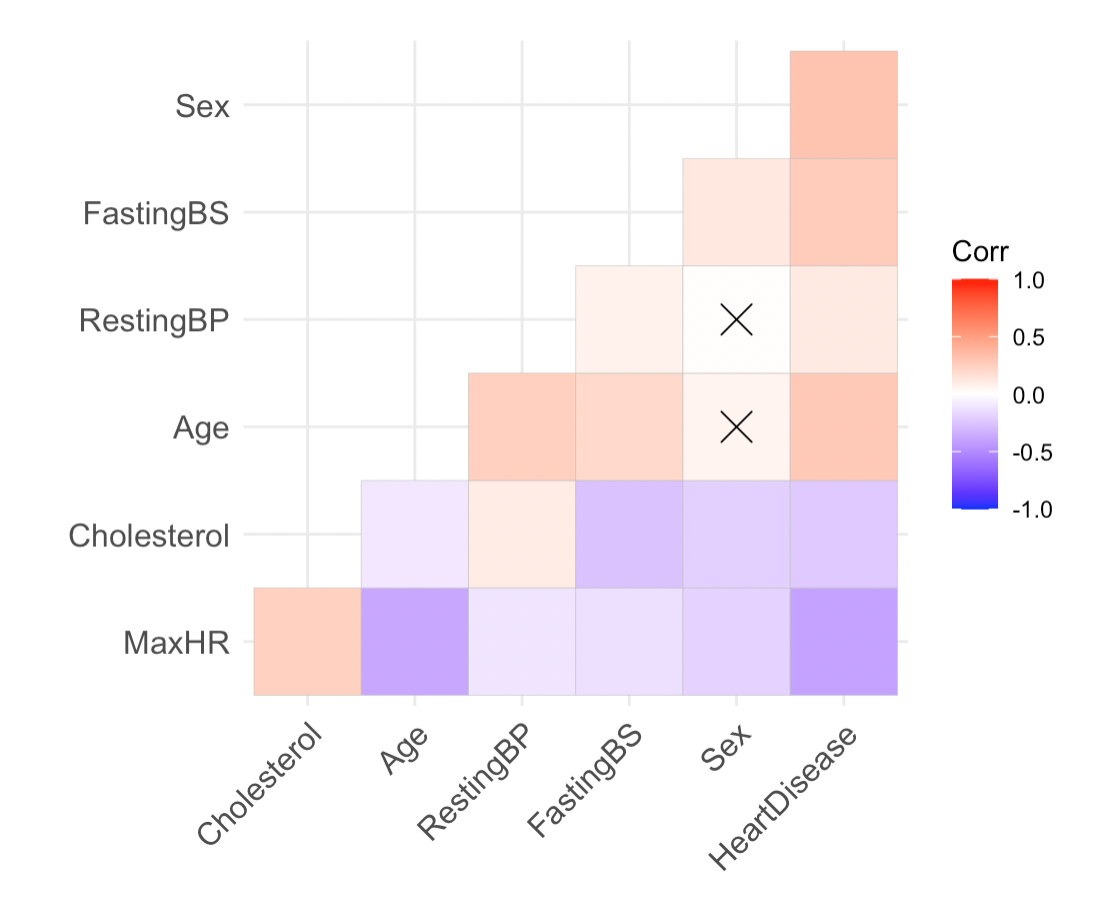
\includegraphics[width=0.5\textwidth]{images/cor.PNG}
	\caption{Correlation Matrix with color encoding}
	\label{fig1}
\end{figure}

\subsection {Distribution of Age}

We then investigate individual predictors by looking at their distributions grouped by heart disease\ref{fig2}. The way to look at the graph is that given an age (x), look at the proportion of people with heart disease to that without heart disease. We clearly see that before 50 years old, more people in the sample did not have heart disease, whereas people of 50+ years tend to have more heart disease. 


\begin{figure}[h]
	\centering
	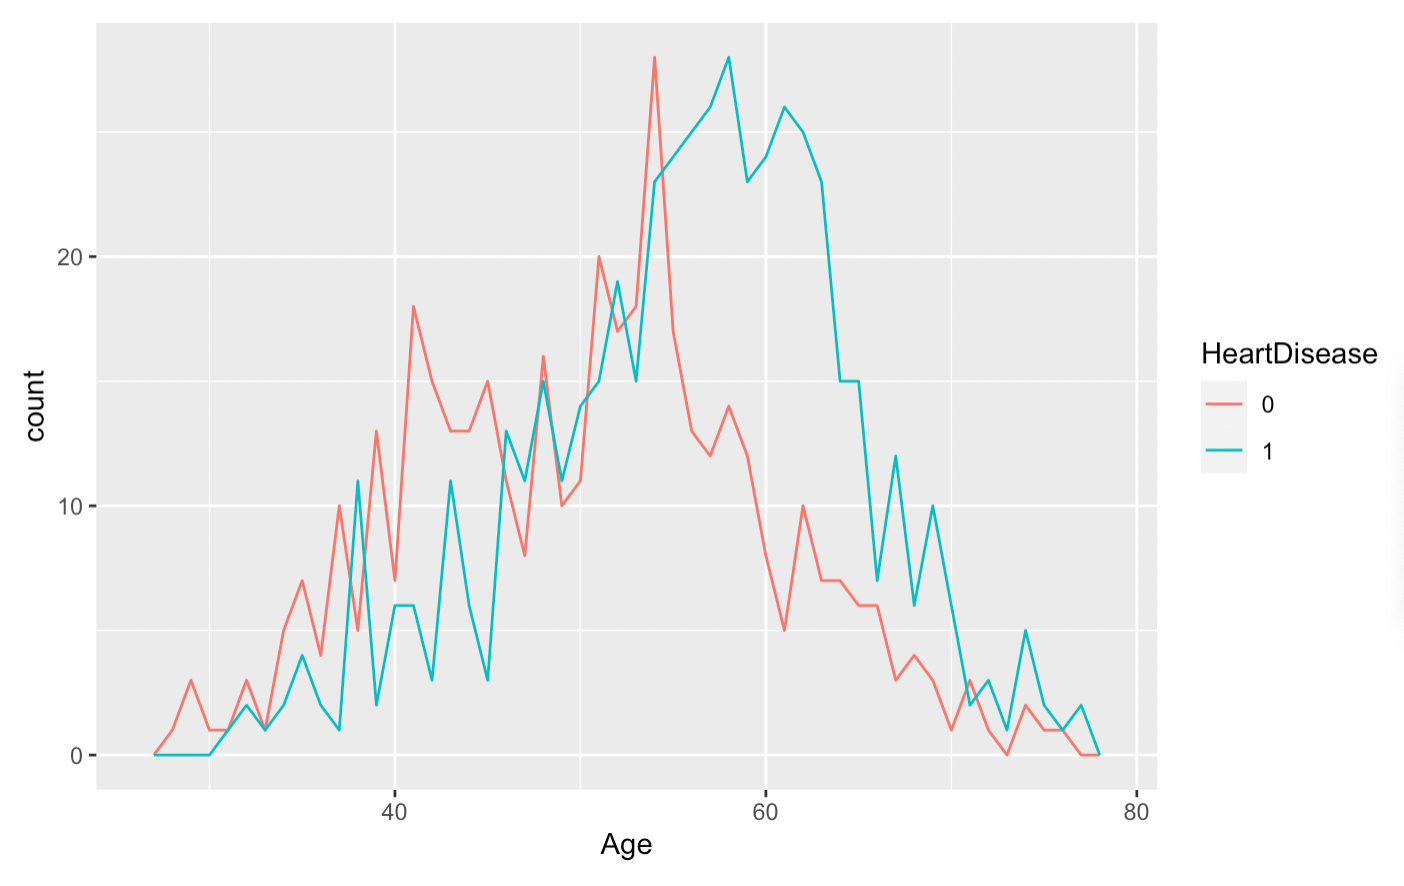
\includegraphics[width=0.5\textwidth]{images/dist1.PNG}
	\caption{Distribution of Age separated by heart disease}
	\label{fig2}
\end{figure}

\subsection {Distribution of Resting Blood Pressure}

For resting blood pressure, the distributions look overlapped a lot\ref{fig2}. However, in later significance testing, we will find that resting blood pressure is still significant predictor. 

\begin{figure}[h]
	\centering
	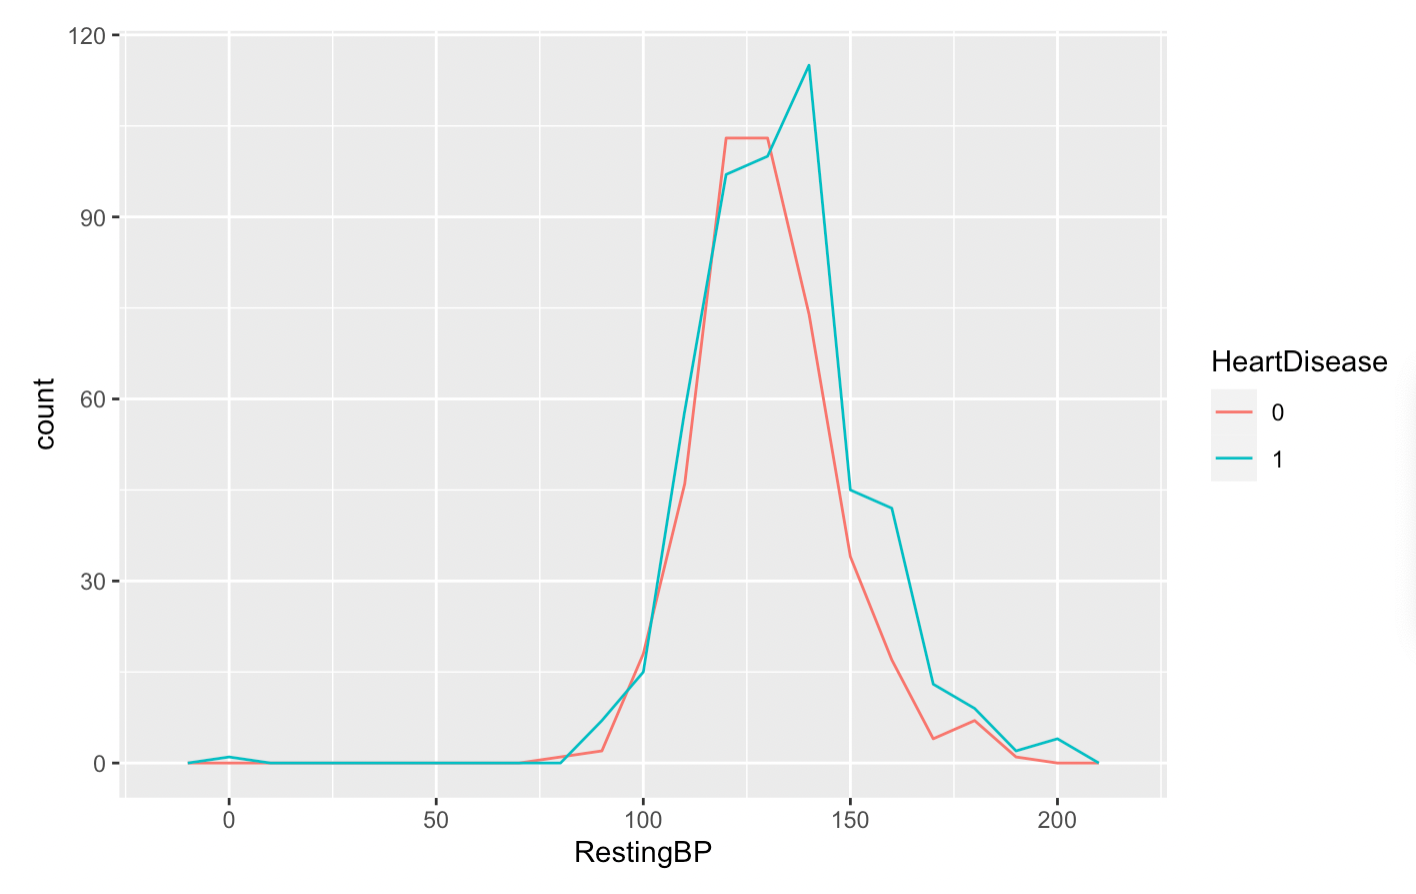
\includegraphics[width=0.5\textwidth]{images/dist2.PNG}
	\caption{Distribution of Resting Blood Pressure separated by heart disease}
	\label{fig3}
\end{figure}

\subsection {Distribution of Cholesterol}

When investigating the cholesterol distribution, we found that there were abnormally large number of 0s recorded in the data, as the huge spikes on the left of the graph indicates\ref{fig4}. Since it is biologically impossible to have a cholesterol level of 0, a healthy cholesterol level is less than 200 mg/dl, we decide that they were missing data and replaced them with NAs. After fixing the data, the new distribution shows a strong, positive relationship between cholesterol and heart disease\ref{fig5}. As a side note, the correlation matrix above included the false 0s, thus showing a negative relationship between cholesterol and heart disease, when in fact it should be positive\ref{fig1}. 

\begin{figure}[h]
	\centering
	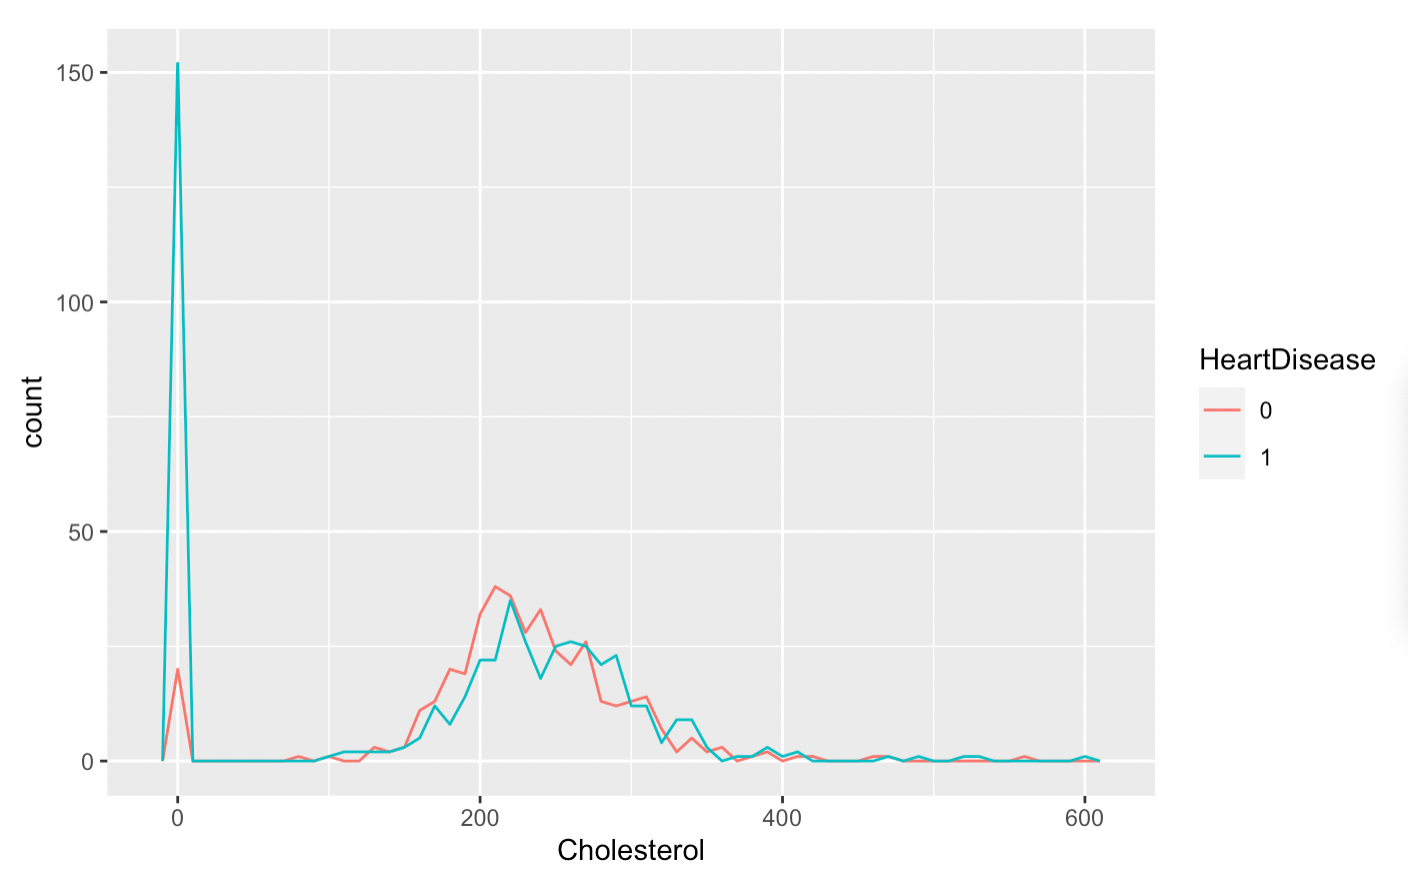
\includegraphics[width=0.5\textwidth]{images/dist3.PNG}
	\caption{Distribution of Cholesterol Before data fixing}
	\label{fig4}
\end{figure}

\begin{figure}[h]
	\centering
	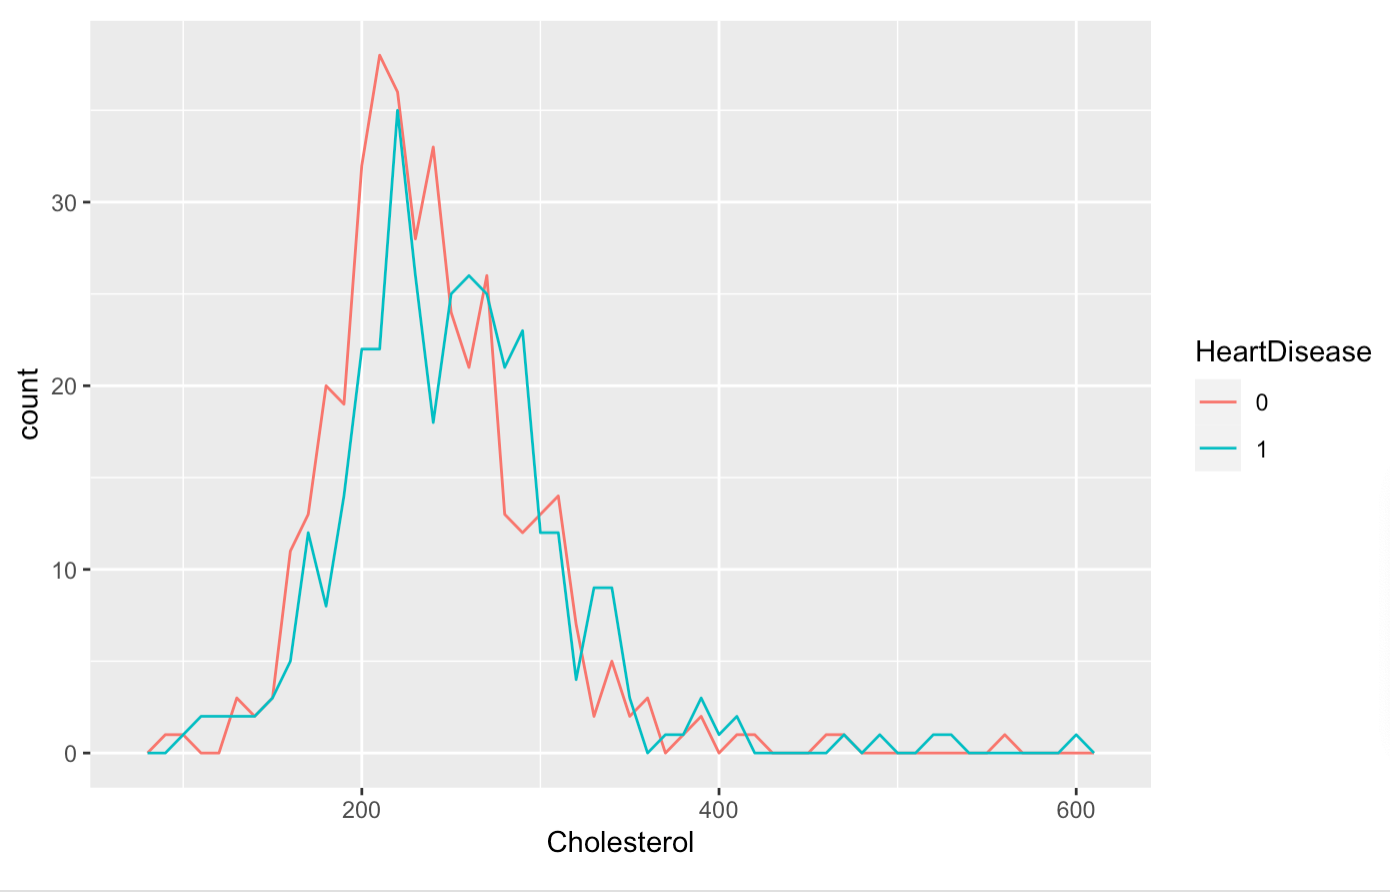
\includegraphics[width=0.5\textwidth]{images/dist4.PNG}
	\caption{Distribution of Cholesterol After data fixing}
	\label{fig5}
\end{figure}

\subsection {Distribution of Max Heart Rate, Sex, and Fasting Blood Sugar Level}

A healthy max heart rate is calculated with the following formula: 220 - Age. For example, a healthy max heart rate for a 70 year old patient would be 220 - 70 = 150 bpm. From the graphs, it seems that max heart rate have a negative correlation with heart disease. For the two categorical variables Sex and FastingBS, we used a stacked dot plot with the dot size representing sample size in that certain group. While males have a 50-50 heart disease ratio, female patients have proportionally significantly fewer heart diseases. For the Fasting Blood sugar level, we can see that when blood sugar level goes beyond 120 mg/dl, the risks of heart failure increase significantly.

\begin{figure}[h]
	\centering
	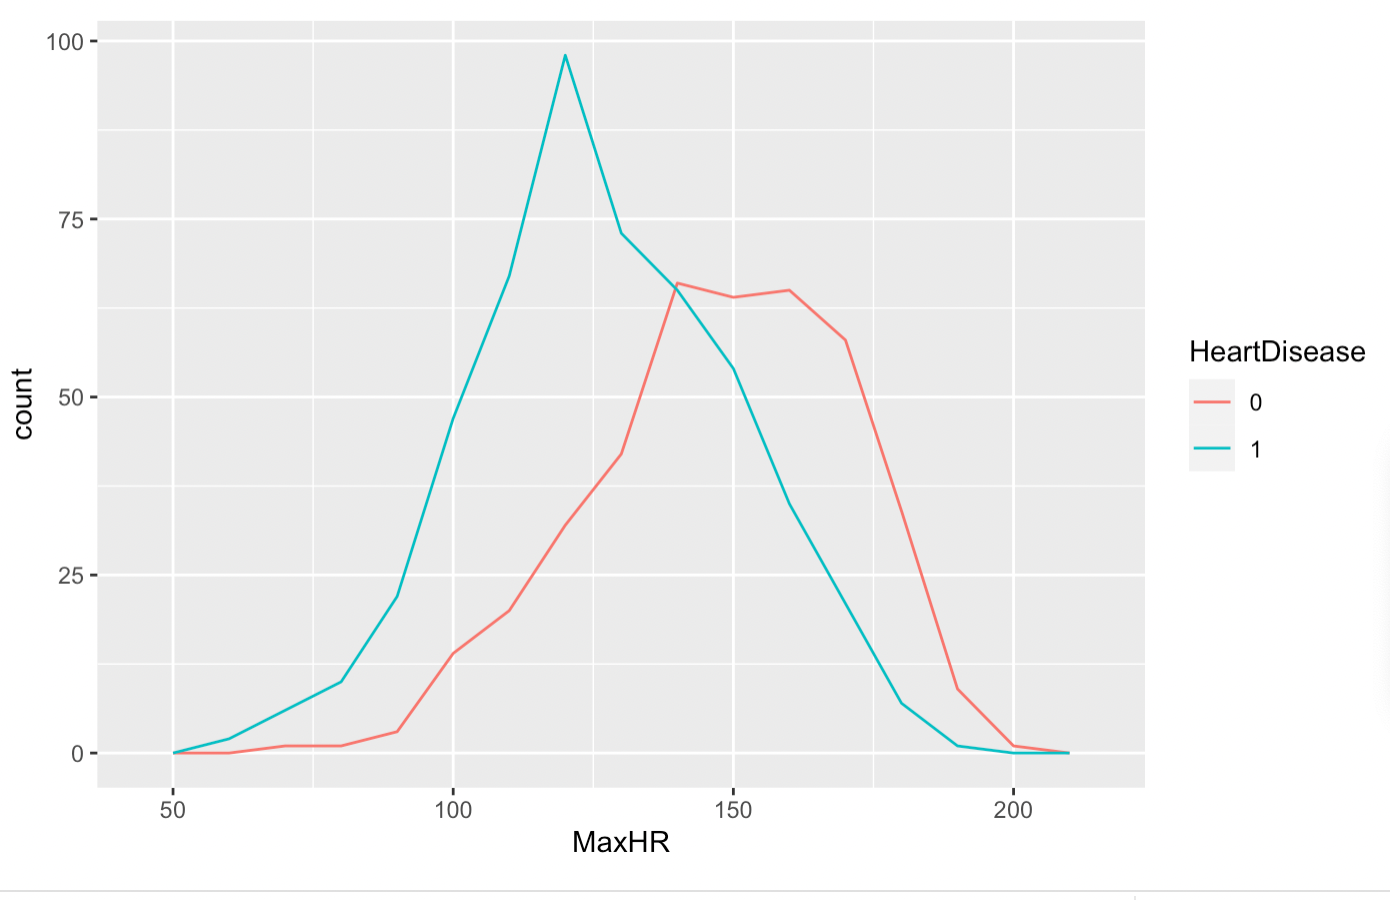
\includegraphics[width=0.5\textwidth]{images/dist5.PNG}
	\caption{Distribution of Max Heart rate}
	\label{fig6}
\end{figure}

\begin{figure}[h]
	\centering
	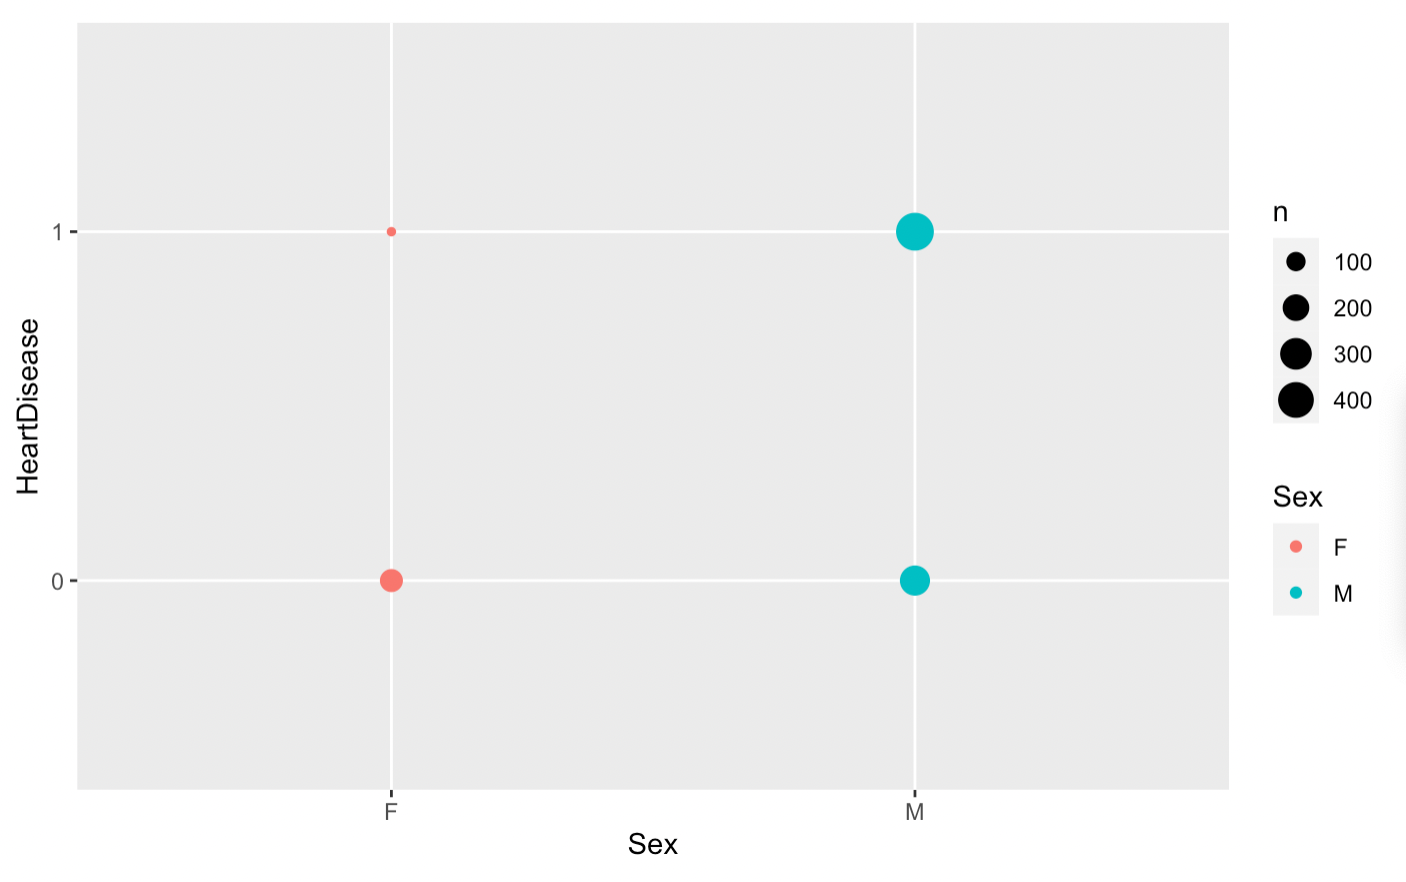
\includegraphics[width=0.5\textwidth]{images/dist6.PNG}
	\caption{Distribution of Heart Failure by Sex}
	\label{fig7}
\end{figure}

\begin{figure}[h]
	\centering
	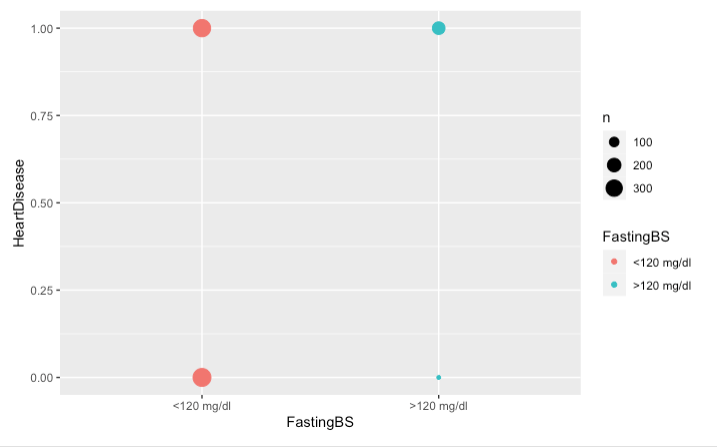
\includegraphics[width=0.5\textwidth]{images/dist7.PNG}
	\caption{Distribution of Heart Failure by Fasting Blood Sugar Level}
	\label{fig8}
\end{figure}

\section{ANOVA}

We use ANOVA to test if the correlation we visualized were significant. We ran ANOVA for each individual predictor and Heart Disease because multi-collinarity might affect the scores if all predictors are ran at once. The ANOVA table shows all predictors are significant\ref{fig9}.

\begin{figure}[h]
	\centering
	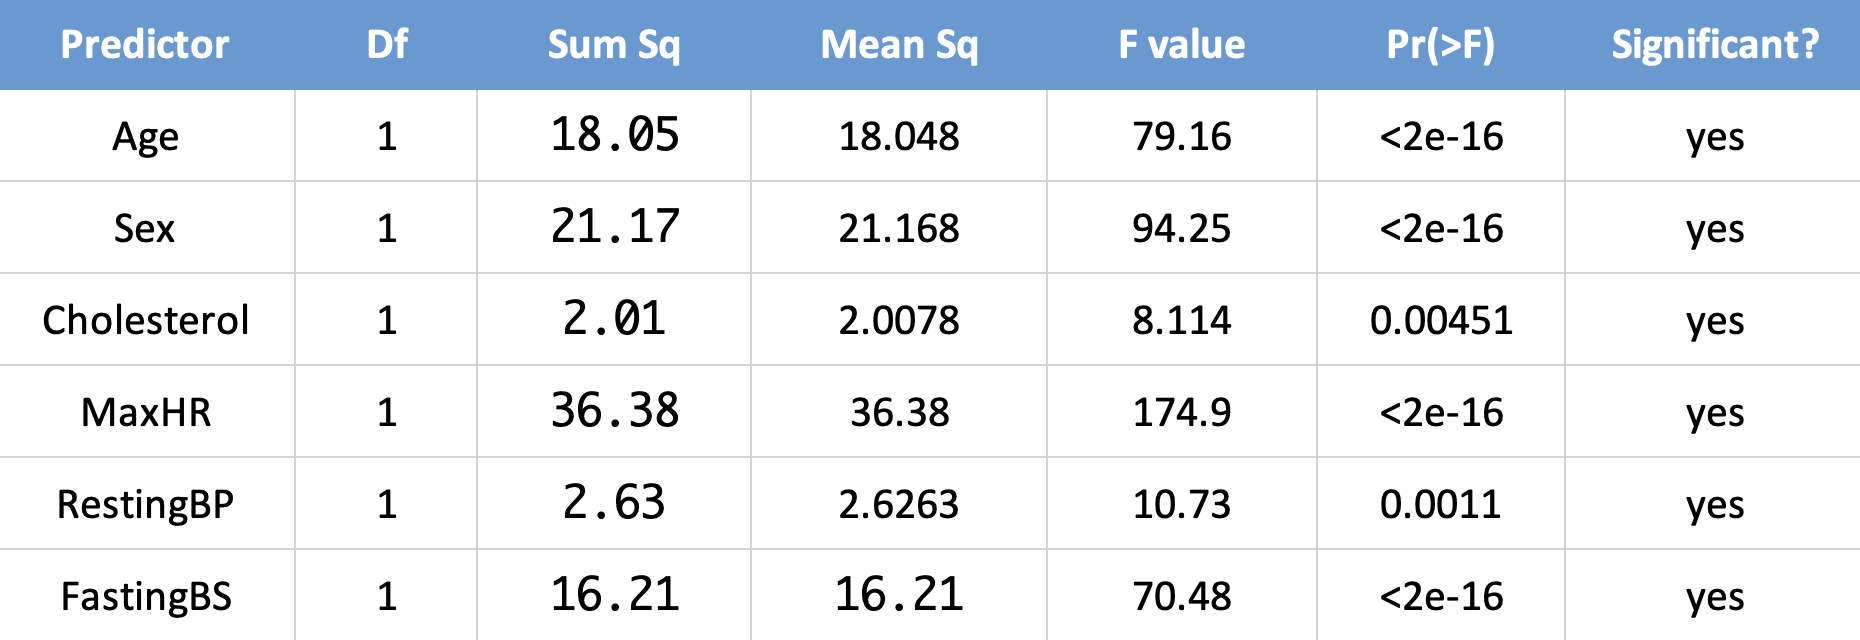
\includegraphics[width=0.5\textwidth]{images/anova.PNG}
	\caption{ANOVA Table}
	\label{fig9}
\end{figure}


\section{Result and Conclusion}
After looking the various predictors within the heart disease data set, we initially created a correlation matrix to find the relation between common symptoms of heart disease and heart disease. Following the correlation matrix, we took a closer at each predictor through an analysis of positive cases and negative cases of heart disease in relation with given predictor. 

Through our findings we can conclude that all six given predictors, Sex, Age, Fasting BS, Resting BP, Cholesterol, and Max Heart Rate, play a large role in indicating heart disease.

Sex: Males are 250\% more likely to get heart disease.
Age: 60+ are 66\% more likely to get heart disease.
Fasting BS: Above 120 mg/dl are 65\% more likely to get heart disease.
Resting BP: Above 145 bpm are 27\% more likely to get heart disease.
Cholesterol: Above 280 mg/dl are 30\% more likely to get heart disease.
Max Heart Rate: Below 150 bpm are 132\% more likely to get heart disease.


\begin{thebibliography}{1.7} 
	\bibitem[1]{Septiawan1} \color{black}
    Kaggle: The Heart Failure Prediction Data Set [Online].Available:https://www.kaggle.com/
    datasets/asgharalikhan/mortality-rate-heart-patient-pakistan-hospital \color{black}
	\bibitem[2]{Septiawan2} \color{black}Heart Disease CDC [Online]. Available: https://www.cdc.gov/heartdisease/index.html \color{black}
\end{thebibliography}
\end{document}